\genHeader

We start with a common step. Unfortunately, it's only a small step, so we do apologize for the white space. In the future, keep an eye out small notes that tell you if and where you can skip ahead. We include ample white space to make the distinction between each of the syntax instructions crystal clear.

\section{Install our plugin for Eclipse}
 
\begin{itemize}
\item[$\blacktriangleright$] Download and install Eclipse for Modelling ``Eclipse Modeling Tools (includes incubating components)''\footnote{Please note that you \emph{have to} install \emph{Eclipse Modeling Tools}, from the Juno download packages, or nothing will work.  Do not choose a different Eclipse package!  Although different versions might work, eMoflon is currently tested for Eclipse Juno and Java 1.7.} from \url{http://www.eclipse.org/downloads/packages/release/juno/sr2} (Fig.~\ref{fig_downloadModelingPackage}).

\begin{figure}[htbp]
	\centering
  	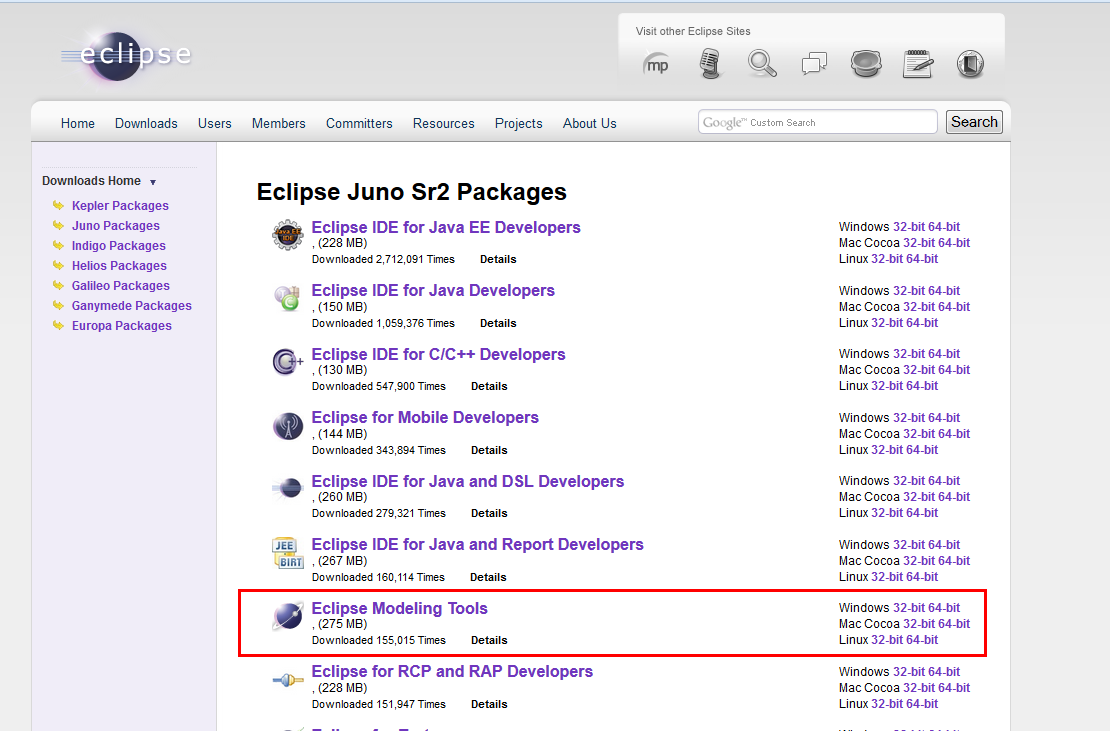
\includegraphics[width=0.86\textwidth]{eclipse_modelingTools}
	\caption{Download Eclipse Modeling Tools.}
	\label{fig_downloadModelingPackage}
\end{figure}

\pagebreak

\item[$\blacktriangleright$] Install our Eclipse Plugin from the following update site\footnote{For a detailed tutorial on how to install Eclipse and Eclipse Plugins please refer to \url{http://www.vogella.de/articles/Eclipse/article.html}} 
\footnote{Please note: Calculating requirements and dependencies when installing the plugin might take quite a while depending on your internet connection.}:
\url{http://www.moflon.org/fileadmin/download/moflon-ide/eclipse-plugin/update-site2}

\end{itemize}